\documentclass{report}

\usepackage[utf8]{inputenc}
\usepackage{biblatex}
\usepackage{dsfont}
\usepackage{mathtools}
\usepackage[colorinlistoftodos]{todonotes}
\usepackage[bottom]{footmisc}
\usepackage{hyperref}
\usepackage{svg}
\usepackage{amsmath}
\usepackage{amssymb}
\usepackage{amsthm}
\usepackage{cancel}
\usepackage{float}

\graphicspath{ {./images/} }

\addbibresource{bibliography.bib}

\newtheorem{property}{Property}


%%%%%%%%%%%%%%%%%%%%%%%%%%%%%%%%
%% SET TITLE PAGE VALUES HERE %%
%%%%%%%%%%%%%%%%%%%%%%%%%%%%%%%%
%             ||               %
%             ||               %
%             \/               %

\def\thesistitle{Designing and implementing a participant login solution for PEP using YIVI}
%\def\thesissubtitle{Why I Definitely Deserve a Fields Medal}
\def\thesisauthorfirst{Giacomo Tommaso}
\def\thesisauthorsecond{Petrucci}
\def\thesissupervisorfirst{prof. Bart}
\def\thesissupervisorsecond{Jacobs}
\def\thesissecondreaderfirst{prof. Erik}
\def\thesissecondreadersecond{Poll}
\def\thesisdate{February 2024}


%             /\               %
%             ||               %
%             ||               %
%%%%%%%%%%%%%%%%%%%%%%%%%%%%%%%%
%% SET TITLE PAGE VALUES HERE %%
%%%%%%%%%%%%%%%%%%%%%%%%%%%%%%%%


%% FOR PDF METADATA
\title{\thesistitle}
\author{\thesisauthorfirst\space\thesisauthorsecond}
\date{\thesisdate}



\begin{document}

\begin{titlepage}
	\thispagestyle{empty}
	\newcommand{\HRule}{\rule{\linewidth}{0.5mm}}
	\center
	\textsc{\Large Radboud University Nijmegen}\\[.7cm]
	
\includegraphics[width=25mm]{in_dei_nomine_feliciter.eps}\\[.5cm]
	\textsc{Faculty of Science}\\[0.5cm]
	
	\HRule \\[0.4cm]
	{ \huge \bfseries \thesistitle}\\[0.1cm]
	%\textsc{\thesissubtitle}\\
	\HRule \\[.5cm]
	\textsc{\large Thesis MSc Cyber Security}\\[.5cm]
	
	\begin{minipage}{0.4\textwidth}
	\begin{flushleft} \large
	\emph{Author:}\\
	\thesisauthorfirst\space \textsc{\thesisauthorsecond}
	\end{flushleft}
	\end{minipage}
	~
	\begin{minipage}{0.4\textwidth}
	\begin{flushright} \large
	\emph{Supervisor:} \\
	\thesissupervisorfirst\space \textsc{\thesissupervisorsecond} \\[1em]
	\emph{Second reader:} \\
	\thesissecondreaderfirst\space \textsc{\thesissecondreadersecond}
	\end{flushright}
	\end{minipage}\\[4cm]
	\vfill
	{\large \thesisdate}\\
	\clearpage
\end{titlepage}

\begin{abstract}
	Polymorphic Encryption and Pseudonimisation (PEP) is both a technology and a project developed at iHub to let researcher collect medical data of people taking part in studies, 
	while preserving their privacy. To do so, it uses ElGamal cipher's properties that allow to re-key and re-shuffle encrypted data and participant identifiers called local 
	pseudonyms. While this system effectively safeguards a participant's privacy, it also makes it non-trivial to design a way for the participants to access their own data: due to 
	PEP's privacy goals, the typical login with email and password is out of the question. This thesis presents a conceptual design for a login system for study participants that
	is in line with PEP's data protection goals and a proof of concept implementation of such system. 
\end{abstract}

\tableofcontents
\pagebreak

\section{Introduction}
Polymorphic Encryption and Pseudonimisation (PEP) is a secure data repository with the goal of storing privacy-sensitive data while preserving the identity and data of participants
in medical studies as much as possible. From a high-level perspective, it looks like a traditional database, because it is structured as a two-dimensional table. But it is not a 
database, as it uses polymorphic encryption to protect the privacy and identity of the study participants, and it has the concept of data cards \cite{pep-blueprint}.\par
To store data in encrypted form, PEP uses the ElGamal cipher. Thanks to ElGamal's re-key operation, it is possible to store the data by an untrusted party even before knowing who
will need to get access to the data. Then the data can be subsequently re-keyed to grant access to the intended person or entity, without exposing the plaintext to the storage provider.
An entity might need a global identifier for the people whose data is stored inside PEP, or to store an already existing identifier but without accessing the original identifier. To
solve this problem, PEP uses ElGamal's re-shuffle operation, that lets derive many identifiers from a "base identifier" without disclosing that base identifier \cite{peppaper}.\par
To enable reproducibility of historical queries, PEP has the concept of data cards. Each piece of data is stored inside a data card which is in turn stored in one of the table's
cells. If the data contained inside a cell needs to be updated, instead of deleting the already existing card, a new data card is generated and stored "on top" of the previous data
card. Thus, each cell contains a deck of cards, and it is possible to see which data a query would have returned in a specific past point in time. \par
PEP's current focus is healthcare, but its general architecture can be used for different purposes. NOLAI \cite{nolai} \cite{pepproject} recently announced that it will use PEP to
collect their research data in the education field. \par
A side effect of PEP's privacy focus is that it didn't ship with a way for study participants, or people whose data is stored inside PEP in general, to get access to their own
data. This constitutes a problem, as article 15 of the GDPR states that "The data subject shall have the right to obtain from the controller confirmation as to whether or not
personal data concerning him or her are being processed, and, where that is the case, access to the personal data [...]" \cite{gdpr-art-15}. 
This work is aimed at finding and developing a solution to this issue.

\section{An introduction to PEP's internals}
PEP's design principles are data and trust minimization. Data minimization consists in giving access to a party only to the data that specific party needs, in order to make
participant identification difficult. Trust minimization consists in dividing PEP's architecture into multiple separate components operated by different parties. The goal is to
prevent a single party from having access to the data: if multiple components need to cooperate to access the data, one doesn't have to trust that each single party will
behave properly. Where this split is not possible, a special component called "transcyptor" keeps an auditable log of the operations performed. This is used to dissuade a party
from misbehaving, as their malicious behavior will be recorded \cite{pep-blueprint}. \par
At the heart of PEP's design, are ElGamal's re-randomize, re-key and re-shuffle operations. To this cryptographic foundation, other elements are added to get a complete functional system. In
particular, PEP uses a form of role-based access control (RBAC) \cite{rbac} to manage users' privileges. It also employs hybrid cryptography for performance reasons and a
distributed architecture to minimize the trust needed in each component. This section will first present a quick recap of the ElGamal cipher and in particular of the re-randomize, re-key and re-shuffle
operations. Then it will briefly discuss PEP's design and focus on PEP's way to manage users' privileges.

\subsection{ElGamal recap}
ElGamal is a public key cryptosystem based on the hardness of computing discrete logarithms \cite{elgamal}. It was originally devised to work on Galois fields, but it has since
been adapted to work on elliptic curves \cite{elliptic-elgamal}. As PEP uses the latter version, this is the one that will be presented here.\par
Assume Alice would like to send an encrypted message to Bob. First, Bob has to choose the domain parameters: a cyclic group composed by the points on an elliptic curve modulo a
prime number, called $E(\mathds{F}_p)$, and a generator for such a group, called $G \in E(\mathds{F}_p)$. He then generates a keypair by generating a uniformly random $b \in \mathds{F}^*_p$ and computing
$B=[b]G$. $b$ is Bob's private key, and $B$ is the public key.\par
Now Alice needs to encode her message $m$ to $M \in E(\mathds{F}_p)$, i.e. a point on the curve. She can then proceed to encrypt it by generating a uniformly random nonce $a \in
\mathds{F}^*_p$ and computing

$$A=[a]G$$
$$C=M+[a]B$$

She then sends the pair $(A, C)$ to Bob. \newline
\par
Bob decrypts the message by computing $M=C-[b]A$ and then decoding $M$ to $m$. This works because, by substituting back the definition for each term of the computation, we obtain
		$$C-[b]A=M+[a]B-[b][a]G=M+[a][b]G-[b][a]G=M$$ 
The last step follows from the commutative property of point addition over an elliptic curve and the existence of the additive inverse.

\begin{property}[Homomorphic property]
ElGamal over elliptic curves is homomorphic with regards to addition: given an encoded message $M \in E(\mathds{F}_p)$ and a point $p \in E(\mathds{F}_p)$, computing $R=M+p$ and
then encrypting $R$ gives the same result as first encrypting $M$ and then summing $p$ to the obtained ciphertext. 
\begin{proof}
This can be easily proven by explicitly carrying the computations in the two cases and observing that they give the same result. Assuming that Alice and Bob choose the same parameters 
as above, this is what Alice obtains during the encryption process in the two scenarios:
\newline \newline
\textit{First scenario: sum and then encrypt}
$$A=[a]G$$
$$R=M+p$$
$$C_1=R+[a]B=M+p+[a]B$$ 
The obtained ciphertext is the pair $(A, C_1)$.
\newline \newline
\textit{Second scenario: encrypt and then sum}
$$A=[a]G$$
$$C_2=M+[a]B$$
$$C_2^{'}=C_2+p=M+[a]B+p$$
The obtained ciphertext is the pair $(A, C_2^{'})$.
\newline \newline
Due to the commutativity of point addition on an elliptic curve, $C_1=C_2^{'}$, thus $(A, C_1)=(A, C_2^{'})$.
\end{proof}
\end{property}

This is the basis for the re-randomize, re-key and re-shuffle operations used inside PEP \cite{peppaper}.
\newline \newline
Given a ciphertext $(A, C)$ where, as before, $A=[a]G$ and $C=M+[a]B$.
\begin{property}[Re-randomization] It is possible to derive a new ElGamal ciphertext that decrypts to the same plaintext under the same key as the original ciphertext, but is different
from the original ciphertext. To obtain this, we pick a random $r \in \mathds{F}^*_p$ and compute $A'=[r]G+A$, $C'=[r]B+C$. The pair $(A', C')$ is the re-randomization of the pair $(A, C)$. \newline
\begin{proof} \label{re-randomization-proof}
		It is trivial to see that the pair $(A', C')$ differs from the pair $(A, C)$, as $r$ is a nonzero element of $\mathds{F}_p$. It remains to be shown that $(A', C')$ decrypts
		to the same plaintext as $(A, C)$, when using the same key. This can be proven by explicitly carrying the decryption process for both ciphertexts. \newline
		\textit{Decryption of $(A, C)$:} \newline
		$$C-[b]A=M+[a]B-[b][a]G=M+[a][b]G-[b][a]G=M$$
\newline
		\textit{Decryption of $(A', C')$:} \newline
		$$C'-[b]A'=[r]B+C-[b]([r]G+A)=\cancel{[r][b]G}+M+[a]B \cancel{-[b][r]G}-[b]A=$$
		$$=M \cancel{+[a][b]G} \cancel{-[b][a]G}=M$$
\newline \newline
In both cases, the decryption process produces the same encoded message $M$.
\end{proof}
\end{property}

\begin{property}[Re-keying] It is possible to obtain a new ElGamal ciphertext that decrypts to the same plaintext as the original ciphertext, but under a different private key. Assuming
that we would like to obtain a new ciphertext encrypted using the public key $[k]B$ from a ciphertext that has been obtained using the public key $B$. We proceed by first
finding $k^{-1} \in \mathds{F}_p$. Then we compute $A'=[k^{-1}]A$. The pair $(A', C)$ decrypts to the same plaintext as the pair $(A, C)$, but under a different private key $kb$.
\newline
\begin{proof}
		Decrypting the pair $(A, C)$ using the private key $b$ gives the encoded message $M$, as shown in the proof of property \ref{re-randomization-proof}. We now show that decrypting the
		pair $(A', C)$ using the private key $kb$ still gives the encoded message $M$. This is again proved by explicitly writing the decryption process:
		$$C-[kb]A'=M+[a]B-[kb]A'=M+[ab]G-[kbk^{-1}]A=M+[ab]G-[b]A=$$
		$$=M+[ab]G-[ba]G=M$$
\end{proof}
\end{property}

\begin{property}[Re-shuffling] It is possible to transform a ciphertext in a way that it decrypts to a re-shuffled version of the message M under the same key, i.e. it decrypts to $nM$ for
some $n \in \mathds{F}_p$. To do this, we compute $A'=nA$ and $C'=nC$. The pair $(A', C')$ decrypts to $[n]M$. \newline
\begin{proof}
		By explicitly writing the decryption process, we obtain:
		$$C'-[b]A'=[n]C-[bn]A=[n](M+[a]B)-[bna]G=[n]M+[na]B-[bna]G=$$
		$$=[n]M+[nab]G-[bna]G=[n]M$$
\end{proof}
\end{property}

\subsection{Data structures}
The main data structure used by PEP is a bidimensional table divided into rows and columns \cite{pep-blueprint}. Each row represents a study participant and each column either the 
results of some medical test or some data used to support PEP's functionalities, like a timestamp used to produce point-in-time queries. The cells pertaining to exam results contain a deck of data cards. \par
Each data card contains the actual results and some metadata. This part of the data card is encrypted using AES-256 \cite{AES-standard} in GCM mode \cite{GCM}. There is then an 
additional field, containing the AES key encrypted using ElGamal over Curve25519 \cite{elliptic-elgamal}. Adopting hybrid Cryptography enables PEP to use ElGamal's properties at a 
performance cost close to the one of applying AES-256-GCM. \par
Using AES-256 instead of AES-128 or AES-192 is not for additional security, as other parts of PEP's design give 128 bits of
security anyway. Rather, the reason is that a 256 bits key has the same size as a point of the used curve, so this makes it straightforward to encode the AES key as a curve point
without having to use any special encoding\footnote{PEP uses the Ristretto technique\cite{ristretto-website} to prevent small subgroup and invalid curve attacks. This approach
encodes curve points to a 32-bytes string, thus it is straightforward to use the same encoding to map 256 bits (32 bytes) AES keys to curve points.}. \par
If the data contained inside a data card needs to be updated, instead of deleting the card a new one is added "on top" of it, overlaying the old data. Subsequent queries will
return the latest data, unless a point in time is specified. In this case, the returned data is the data recorded in the data card that was on top of the deck at that specified
time.

\subsection{Pseudonyms}
As part of the registration procedure, each participant gets assigned a participant identifier, also known as PEP ID. This identifier is not used directly, but instead it serves as a basis to generate
local pseudonyms. These pseudonyms do not depend solely on the participant identifier, but also on the usage context: different studies involving the same participants or different
researchers accessing the same dataset will get different local pseudonyms. This is useful to prevent combining data across different datasets \footnote{It is still possible to
link different local pseudonyms to the same participant by comparing bit-by-bit complicated pieces of data, like brain scans, that are unlikely to be the same for different people. To 
mitigate this possibility, users have to sign an agreement that forbids them to do such comparison.}. These local pseudonyms are obtained by encrypting the participant's identifier 
using ElGamal, and then applying the re-shuffle operation \cite{pep-blueprint}. \par
Sometimes it is necessary to generate an identifier to link a participant to a data source outside PEP. This happens during the collection of samples, e.g. blood samples, to then
perform some analysis in a laboratory. In these cases, researchers need an identifier to put on those samples to then be able to link the results to the correct participant, but
without leaking the participant's identity to the laboratory performing the analysis. Furthermore, for practical reasons, these identifiers need to be short enough to fit on a printed label. To do this, PEP is able to generate short
pseudonyms. These short pseudonyms aren't derived from the participant identifier, and are instead generated as a random number concatenated with a checksum to prevent
transcription errors. These short pseudonyms are then recorded inside a specific column related to the test they are used for, e.g. for a blood test the column storing the short
pseudonyms printed on the blood vials could be called ShortPseudonym.Visit1.Blood  \cite{pep-blueprint}.


\subsection{CRM}
While technically not a part of PEP, using PEP also entails using a customer relationship management (CRM) software as part of logistic procedures involving study participants. In fact, 
after reading the previous section, a question arises naturally: if a nurse or doctor is collecting some sort of samples from study participants to be then sent to a laboratory for 
analysis, and has a set of printed labels with the short pseudonyms generated by PEP, how can he know which is the correct label to apply to each sample? \par
To answer this question, we need to take a step back and briefly describe what happens when a participant is accepted for a study. Let's say that Alice is willing to take part to a
medical study as a study participant. After an initial evaluation to check her eligibility for the study, she gets accepted. At this point, she gets registered for the study. As
part of the registration procedure, PEP generates a PEP ID in the form of a unique pseudorandom number. This identifier is then stored inside the CRM alongside personally
identifying information such as full name and date of birth. This is needed for two purposes: it enables the assessors\footnote{An assessor is a person collecting data from
participants} to verify the identity of the participant during the visits and enables re-identification if this is required because of incidental findings. This answers our
question: when Alice presents herself to a visit where samples are collected, the doctor checks in the CRM what is her PEP ID. Then, using the PEP ID, he can get from PEP the short
pseudonym that was previously generated for the sample that he is going to collect, thus he is able to label it correctly. Only assessors need to be able to link the identity of
study participants to their PEP ID. To keep researcher accessing that data later via PEP from knowing the participants' identities, they are not allowed access to the CRM, the
PEP ID column inside PEP and the columns containing the short pseudonyms, as they don't need these information to perform their research anyway.\par
Currently, the CRM used in combination with PEP is Salesforce \cite{salesforce-website}.


\subsection{PEP servers}\label{pep_servers}
Here is a list of the main server components of PEP. The access manager mentioned here is a piece of software, and should not be confused with the access administrator role mentioned
later, i.e. a person with the right to give users access to the datasets defined by the data administrator.
\begin{itemize}
		\item Storage facility: stores the table and the data cards.
		\item Access manager and transcryptor: issue tickets and keep the access rules. Additionally, the transcryptor keeps an auditable log of the issued tickets.
		\item Key server: checks authentication tokens and signs users' PEP certificates.
		\item Authentication server: keeps the users list and generates authentication tokens. 
		\item Registration server: generates the participant identifiers and the short pseudonyms.
\end{itemize}


\subsection{Data access} \label{data_access}
This and the next section mention PEP users. These are in principle (and, before this thesis work gets implemented, also in  practice) different from study participants. A PEP user is
someone that interacts with PEP, while a study participant is someone taking part in a medical study as a data contributor. \par
To be able to interact with PEP's table, a user needs a ticket granting the correct permissions for the required operation. PEP implements a way to specify access rules for
specific user groups, and then a specific user is assigned to a group. These rules are then used to determine whether to grant a ticket for a specific operation or not. This
constitutes a form of role-based access control \cite{rbac}. \par
To be able to bootstrap this permissions system, it is needed that someone has the right of writing rules for access groups, to specify access groups and to add users to groups. For 
this reason, PEP has two builtin access groups: "Data Administrator" and "Access Administrator" \cite{pep-blueprint}. A member of the former group is called a data administrator, and 
has the permissions needed to modify columns, column groups, and participant groups. A member of the latter group is called an access administrator, and has the right to modify the 
access rules used to issue tickets, modify and read the user list to issue authentication tokens, and manually issue authentication tokens. These two roles are given to distinct people, 
so that they would need to collude to access a specific piece of data. \par
Let's assume that the data administrator would like to access the results of a participant's blood test. First of 
all, it is important to stress once again that PEP's table doesn't contain the names of participants. Study participants are only identified via their participant identifier, and the 
pseudonyms that are derived from such identifier. These are random numbers that don't carry any information regarding a participant's identity. So the data administrator can't access 
the data of a specific person he knows, but could still try to access the data corresponding to a specific pseudonym or PEP ID. Since the data administrator is able to create new user 
groups, he could create a new group containing the participant he would like to spy on, but he can't give himself access to this newly created group. To accomplish this, he needs to 
ask the access administrator. If the access administrator agrees, he can now access the participant's data. In the case the data administrator already has read access to a participant 
group, he could read the data of the participants inside that group and add the participant he is interested in to such group. But this means that the access administrator gave him 
read access to such participant group in the past, and there is no reason why a data administrator should have read access to participants' data. So the only case when this can happen 
is if the access administrator is complicit in accessing participants' data. \par
Let's now consider the case of the access administrator willing to access some specific participant's data. 
He can't create a new participant group containing that participant, so he needs to ask the data administrator to do that for him. If the data administrator accepts and creates such 
group, he can now give himself read access to that group's data, thus obtaining access to the participant's data. But an access administrator could still give himself access to already 
existing groups, including one that already contains the participant he is interested in. To mitigate this problem, PEP employs an architectural solution: there are two separate
servers that need to collaborate to issue a valid ticket granting access to a piece of data. The first is the access manager, and the second is the transcryptor. The access manager's 
role is to apply the rules defined by the access manager, while the transcryptor keeps an auditable log of the issued tickets.\ref{pep_servers} This should dissuade the access 
administrator from misbehaving, as the tickets he uses to access the data will be logged.


\subsection{Authentication and authorization}
PEP's servers are authenticated using TLS certificates. Clients instead authenticate themselves to the servers using PEP certificates \cite{pep-blueprint}. This is different from
TLS' mutual authentication mechanism, as the client signs a request which is then transmitted over TLS. Such signed request is logged by PEP's transcryptor server for auditability. In
both cases, the certificates are X.509 certificates \cite{X.509} issued by the key server using PEP's root certificate \cite{pep-blueprint}. \par
PEP user certificates expire after a limited time and are generated on-demand during a procedure called enrollment. 
There are two ways a user can obtain a PEP certificate. In the first scenario, users authenticate themselves using an authentication token, and generate a certificate that is then
signed by PEP. The token is generated and given them by the access administrator, who also performs the user identification. \par
In the second scenario, a program requests an authentication token for the user using an HTTP API endpoint. In this case, the actual identity verification is done using the SAML 
standard \cite{sstc-saml-core-errata-2.0-wd-07} and SURFconext \cite{surfconext} as an identity provider. Once the user's identity is established, its access rights are determined by 
looking up a user list to determine the user's membership of any access group. 

\subsubsection{SAML}
Security Assertion Markup Language (SAML) is a security standard used to authenticate users and supporting Single Sign On (SSO) \cite{sstc-saml-core-errata-2.0-wd-07}. It defines
the syntax and semantics for XML-encoded assertions regarding authentication, attributes, and authorization of a subject (an entity that is usually a user, but could in principle
be a software component, a device or an entire organization) to other entities. It also defines protocols to exchange these information. SAML supports a number of usage scenarios, those 
relevant for PEP's infrastructure are called "Identity Federation" and "SP-Initiated SSO". \par
The SAML specification calls "Identity Federation" the scenario where two independent parties form an agreement about how to refer to a specific user that interacts with both
parties. Only one of the two parties needs to be able to authenticate the user, and the other party will trust a SAML assertion generated by the first party about the user's identity. \par
"SP-initiated SSO" stands for "Service Provider initiated Single Sign On" and is the procedure through which a service provider asks an identity provider to authenticate a user on
its behalf. The identity provider will follow some procedure to perform the user authentication and, if the authentication is successful, will generate a SAML assertion containing
the user's federated identity. For this scenario to work, the service provider and the identity provider need to have established a federated identity for the user in the past.\par
As anticipated at the beginning of this section, PEP uses this two scenarios to authenticate (programs used by) users via an HTTP endpoint. The (program used by the) user first contacts 
the HTTP endpoint to request an authentication token. It is then redirected to SURFconext's identity provider and presented a login page. The user attempts to login and, if the login is 
successful, the identity provider generates a SAML assertion containing the user's federated identity. The user forwards this assertion to PEP's authentication server that proceeds to 
check this assertion and, if valid, generates the corresponding authentication token that is then sent to the user. This token is used during further interaction with other PEP 
components. See image \ref{bpmn-authentication-flow} for a BPMN diagram representing PEP's authentication flow.

\subsubsection{RBAC}
Role-Based Access Control (RBAC) is a form of non-discretionary access control that, contrary to Mandatory Access Control (MAC), is not based on multilevel security requirements \cite{rbac}. \par
Compared to Discretional Access Control (DAC), RBAC does not let users transfer their access rights to someone else. Compared to MAC, instead of deciding whether to grant a user access 
to a resource or not based on the confidentiality level of the resource and the user's security clearance, RBAC makes decisions based on the user's role within an organization and a set 
of rules specifying each role's access level. \par
DAC is typically used in the context of Operating Systems. The reason is that it is reasonable to assume that the creator of a file also owns that file, thus can decide who is
allowed to access it. MAC is instead usually employed in the military sector, as typically in that scenario documents are classified based on their confidentiality, and people are
given access rights based on their level inside a rigid hierarchy\footnote{By rigid hierarchy I mean that, given two people with different roles, it is always clear which of the two 
has a superior role. Compare this with the situation inside a company, where two people can have different roles, but without one being higher in the company's hierarchy compared to
the other.}. RBAC is often used in the commercial sector as the situation there is often in-between the scenarios of DAC and MAC: on one hand, employees working on a document
typically don't own it, so they should not be able to decide on their own to give access to that document to other employees. On the other hand, a company doesn't have a strict
hierarchy, and a person's level of access to resources depends more on this person's role inside the company rather than this person's place inside the company's hierarchy. This is
also the case of PEP: researchers working inside different projects are at the same hierarchical level, but must be given access only to the data pertaining their own research. In
other words, the data pertaining some research is not more or less secret than the data pertaining another research, but it can happen that researchers with the rights to access
the data of some study should not be allowed to access the same kind of data but pertaining to a different study. At the same time, a researcher should not be allowed to transfer his
own access level to another user. \par
As mentioned in section \ref{data_access}, PEP implements RBAC by having a "data administrator" and an "access administrator". The first defines a set of access permissions and the
second links users with these rights. The act of defining access permissions is equivalent to defining roles, and the act of linking these rights with users is equivalent to assigning
roles to users. 


\subsection{Data Access Flow}
This section presents a concise overview of PEP's current flow to access the data. For the detailed message exchange that happens in each of the following phases, see
\cite{pep-blueprint}.

\subsubsection{Authentication}
The data access flow starts with the user contacting PEP's authentication server. It redirects the user to the SurfConext identity provider, and the user has to authenticate to that 
service. If the authentication is successful, the identity provider generates a SAML assertion that the user's browser forwards to PEP's authentication server. Based on the
SAML assertion, the authentication server sends the user an authentication token.

\begin{figure}[H]
	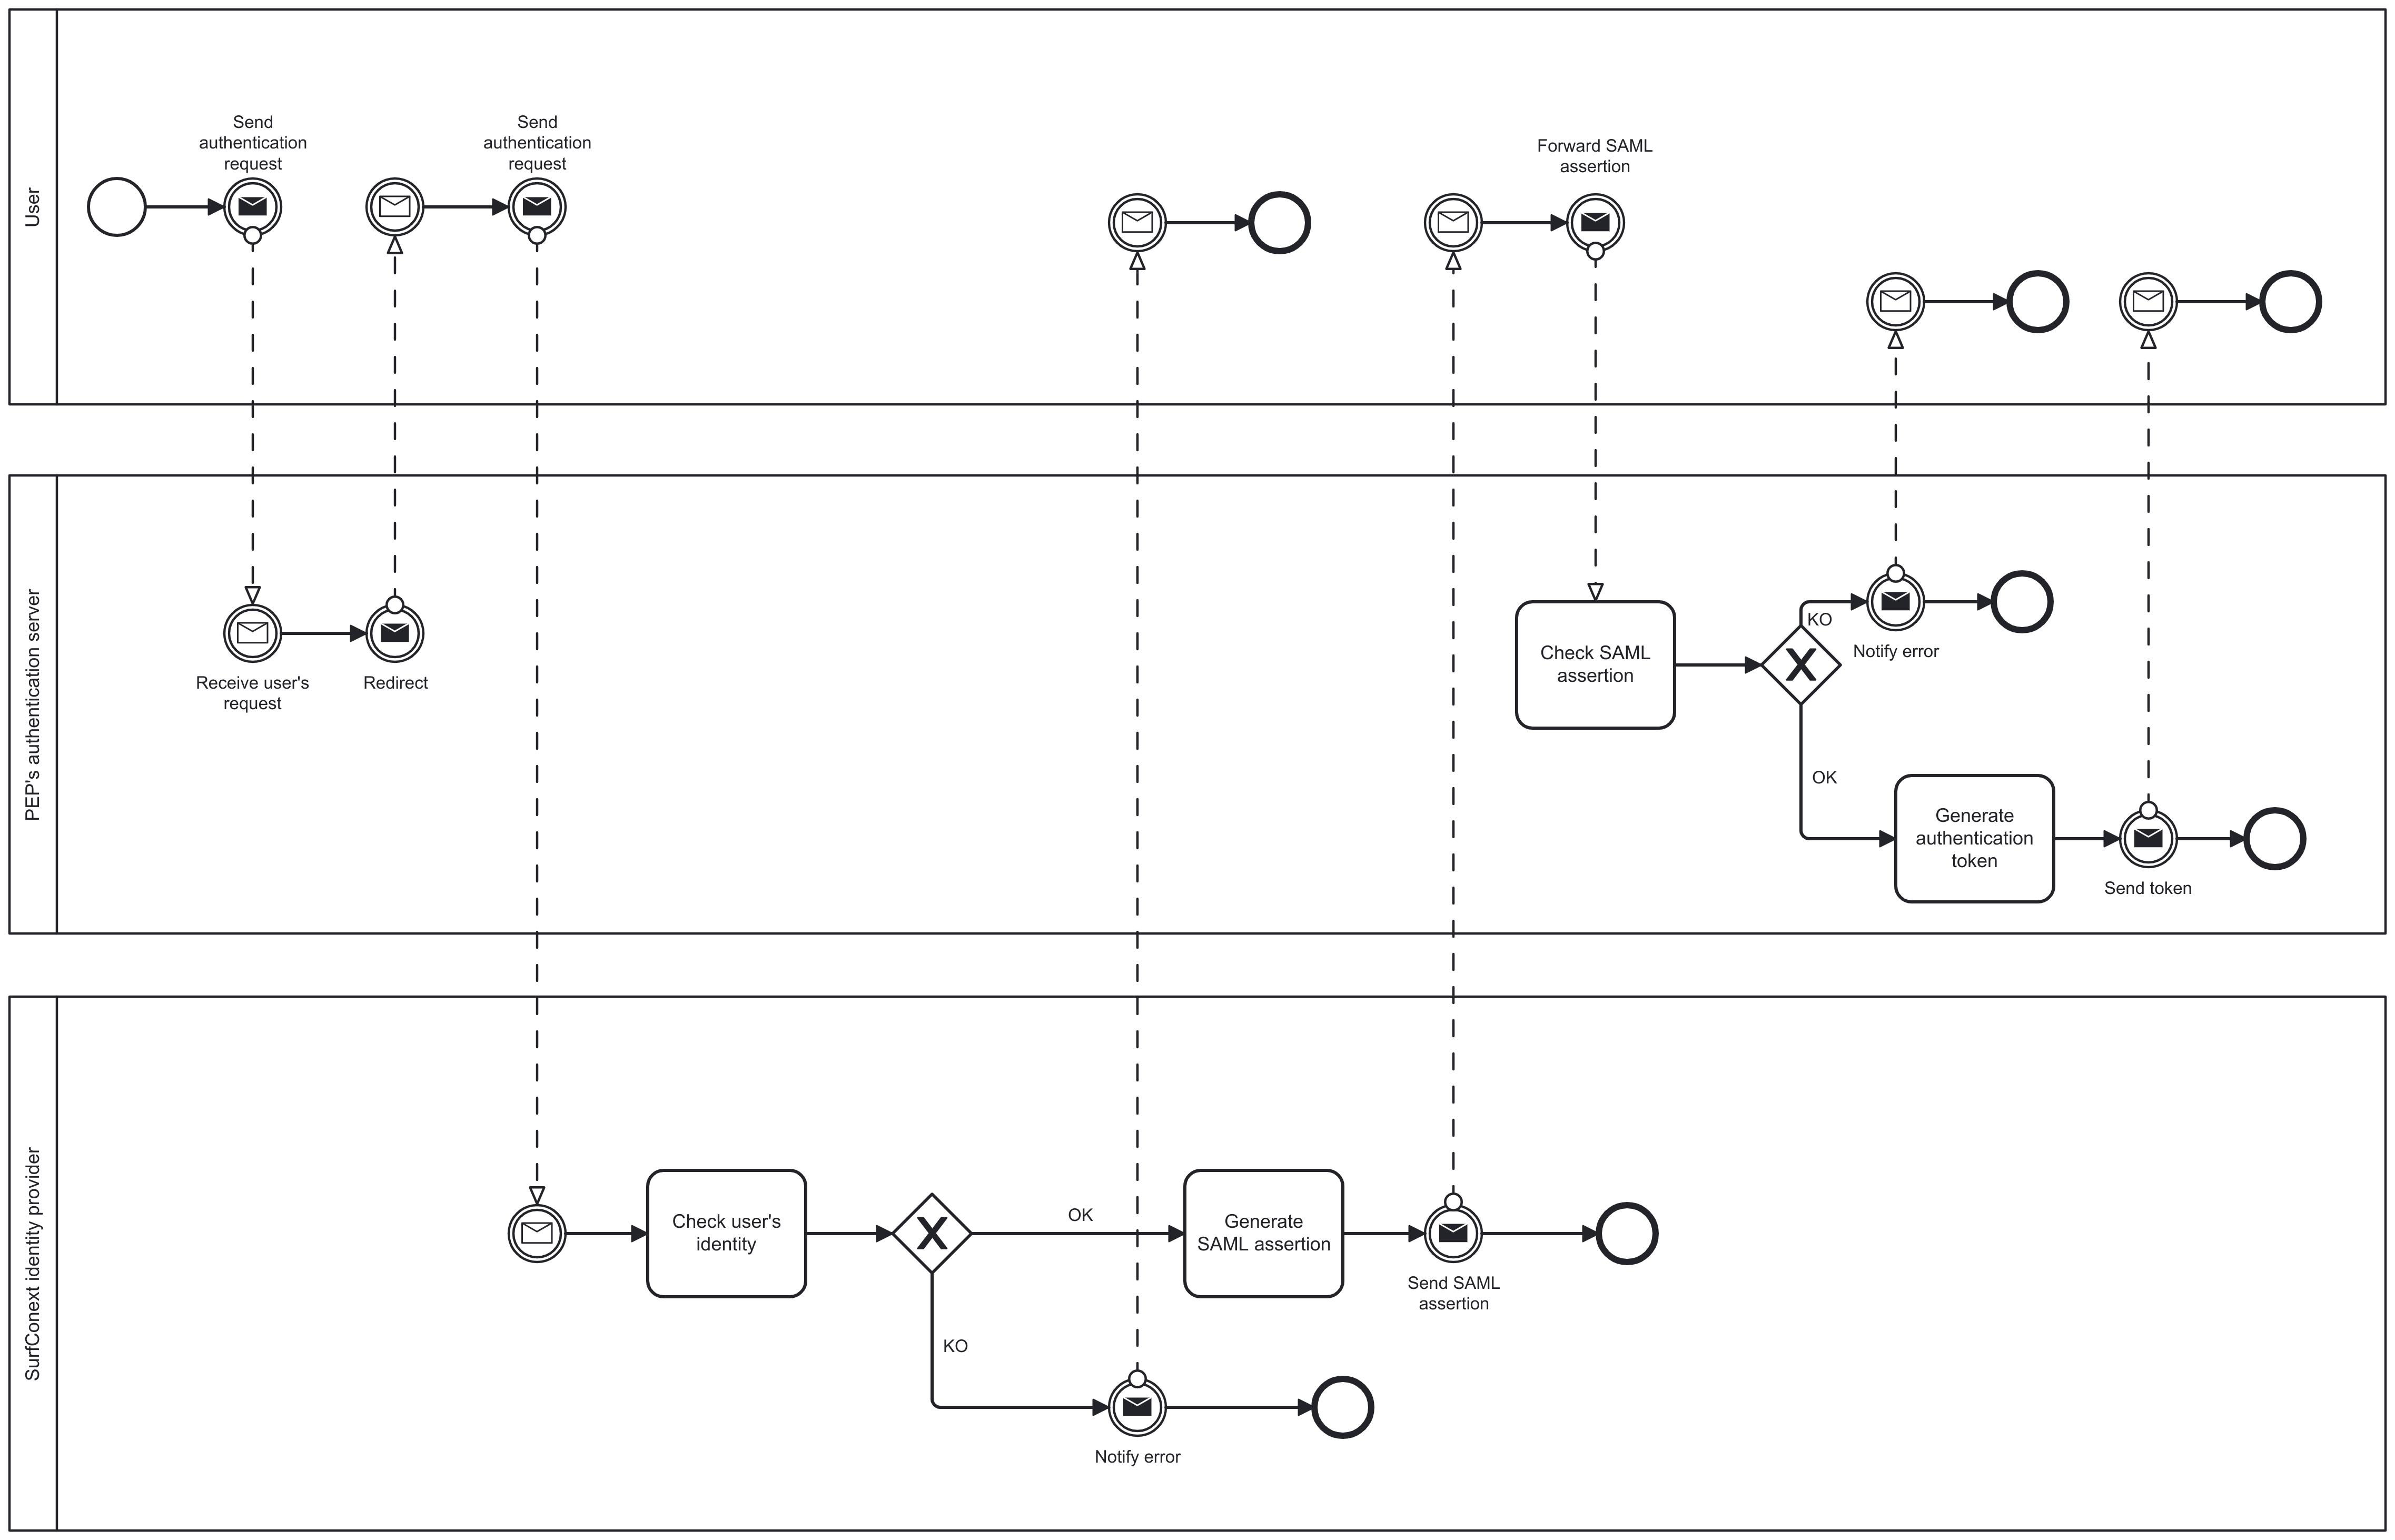
\includegraphics[scale=0.1, angle=-90]{authentication.png}
	\caption{PEP's authentication flow as a BPMN diagram}
	\label{bpmn-authentication-flow}
\end{figure}

\subsubsection{Enrollment}
In this phase, a user obtains a PEP certificate and his own ElGamal private key needed to decrypt the data. \par
It starts with the user contacting PEP's key server and presenting an enrolment request. This request contains the user's authentication token and a certificate signing request.
The certificate signing request is a X509 certificate, minus the signature. If the token is valid, the certificate signing request is signed by the key server and becomes a valid PEP 
certificate. Then the user contacts the access manager and transcryptor servers, to obtain the key components. These key components are two factors that, when ,multiplied together,
generate the user's private key. These factors are split between two servers, so none of the two has knowledge of the user's private key. The user multiplies the two factor,
obtaining its own key.

\begin{figure}[H]
	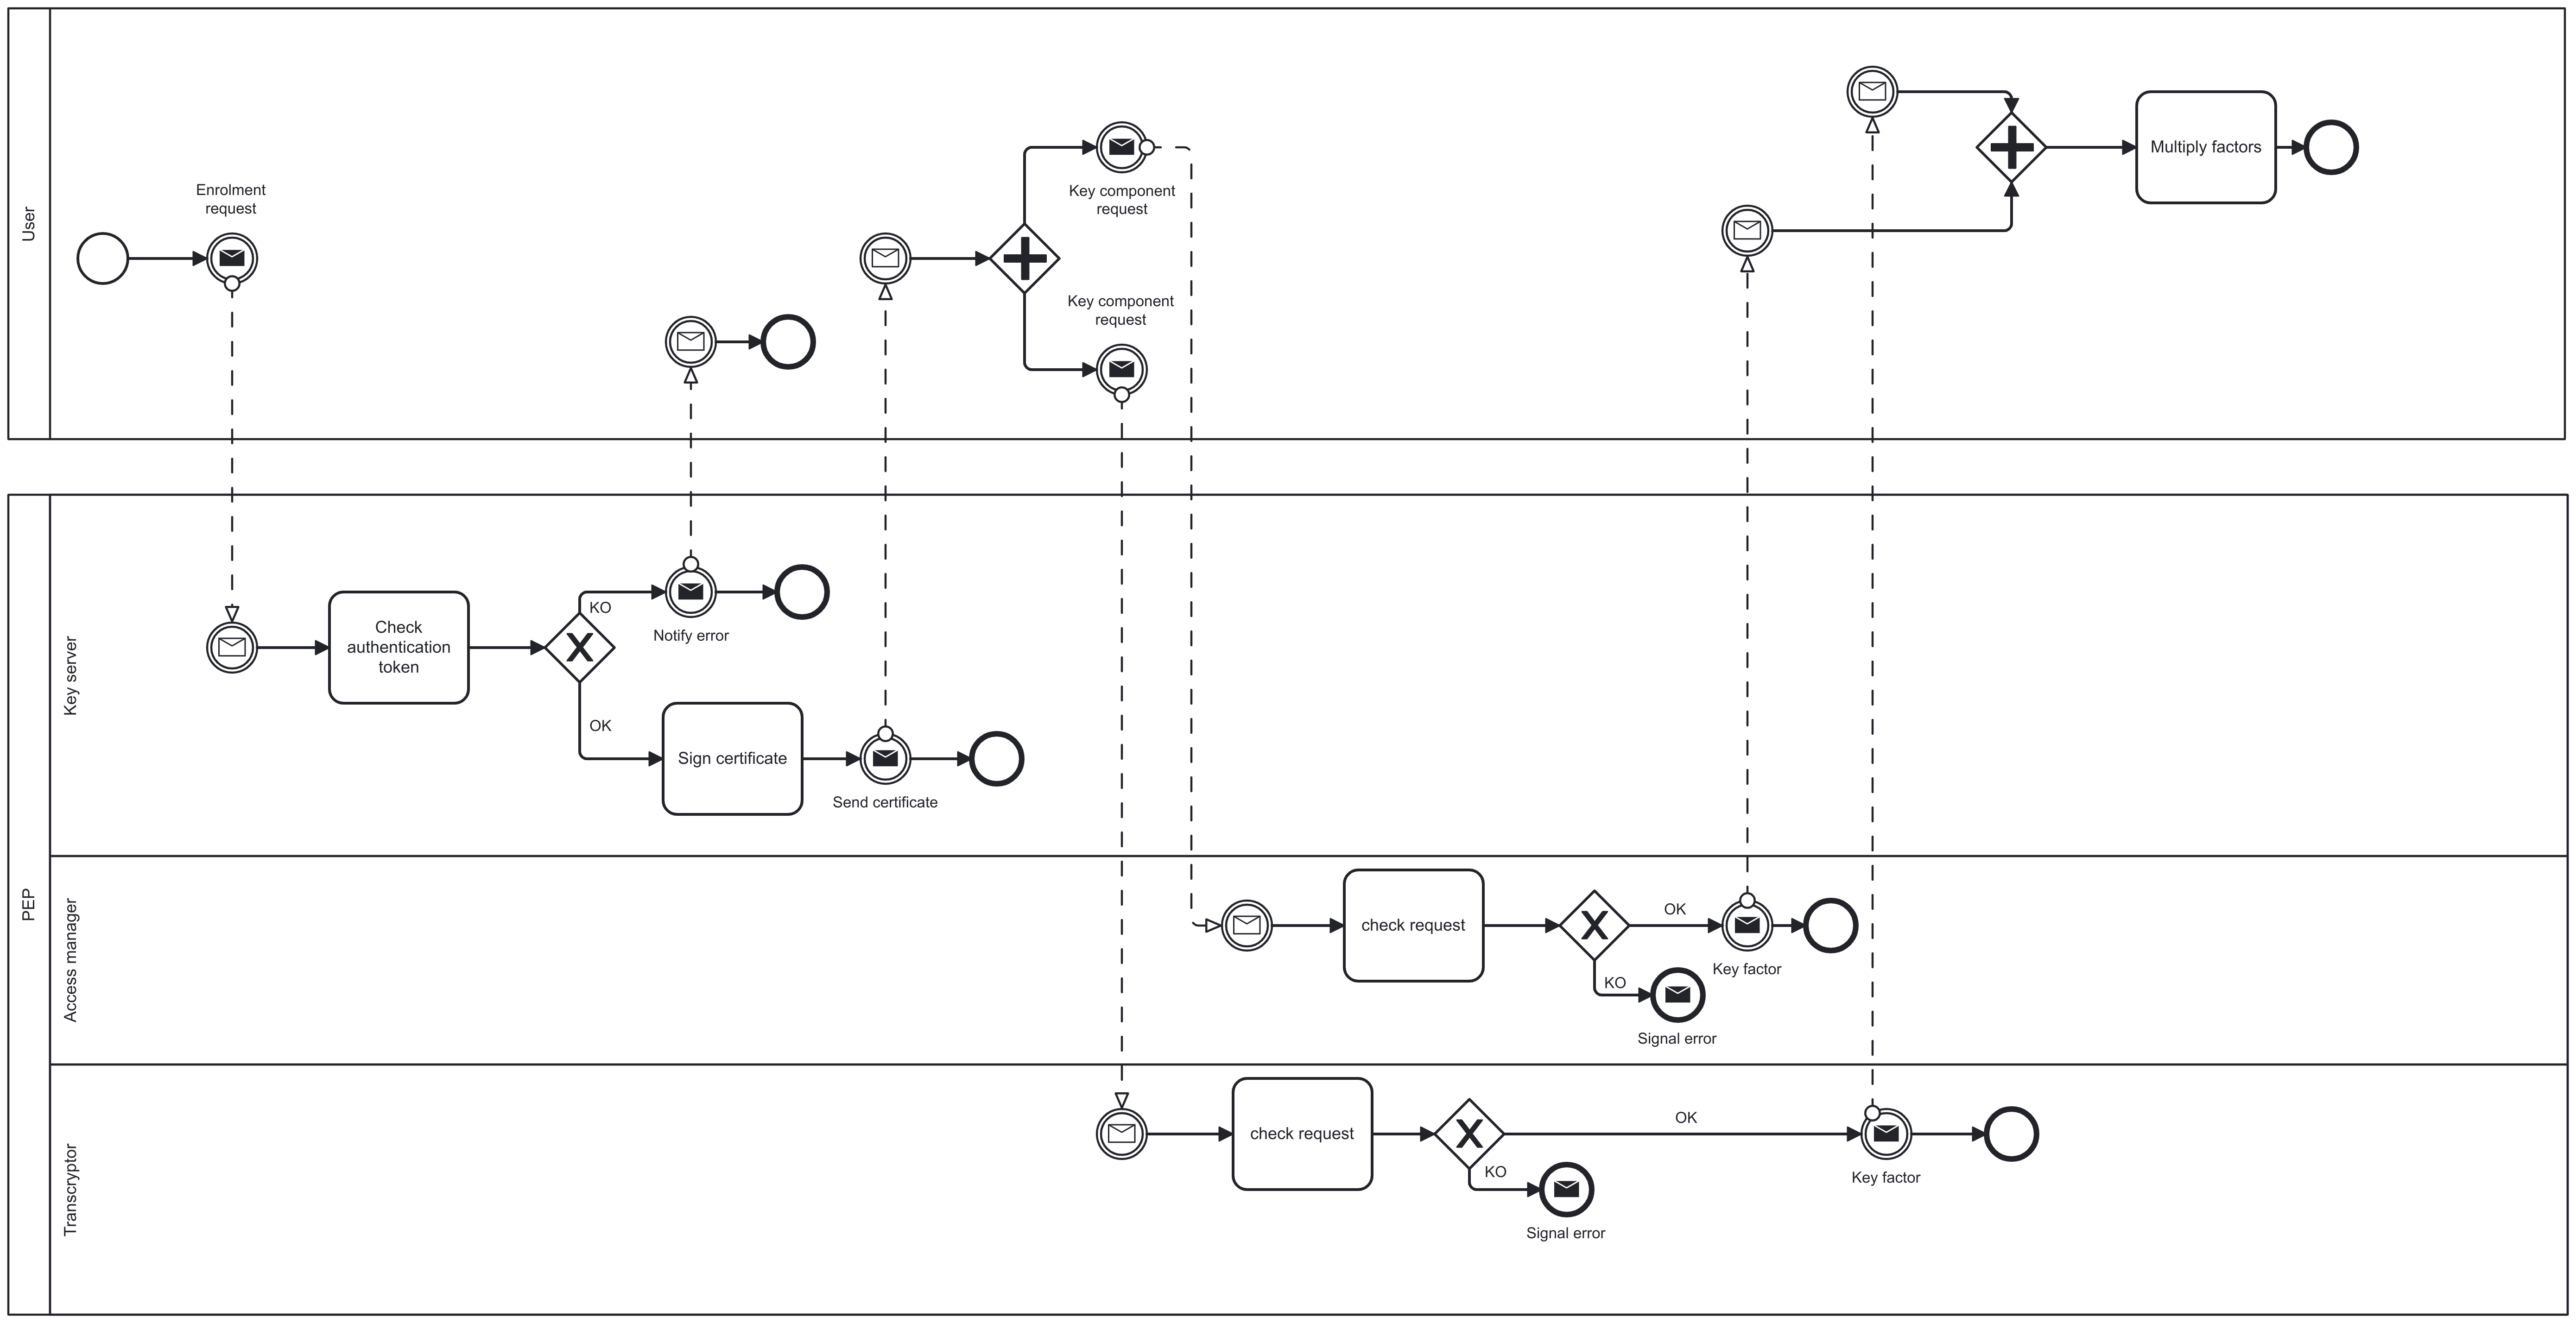
\includegraphics[scale=0.1, angle=-90]{enrollment}
	\caption{PEP's enrollment flow as a BPMN diagram}
	\label{bpmn-enrollment-flow}
\end{figure}



\section{How to give access to study participants}
\subsection{Failed attempt}
At the beginning of this work, I considered many possible solutions, that either turned out to not respect PEP's privacy standard or were deemed risky by the PEP team. Other
solutions, instead, while feasible in theory, failed in practice. This section briefly presents one of those of the latter category, as it would have made for a clean solution that
nicely integrates with the rest of PEP's architecture. Even though this attempt at a solution did not work out, some elements of it were used as part of the working solution
presented later.\par

\subsubsection{Design choices}
As PEP already uses the SAML standard \cite{sstc-saml-core-errata-2.0-wd-07} for authentication, it would be natural to implement a SAML identity provider using YIVI \cite{irma-app}.
Here is a BPMN diagram of the process that would be required to register a new study participant.

\begin{figure}[H]
	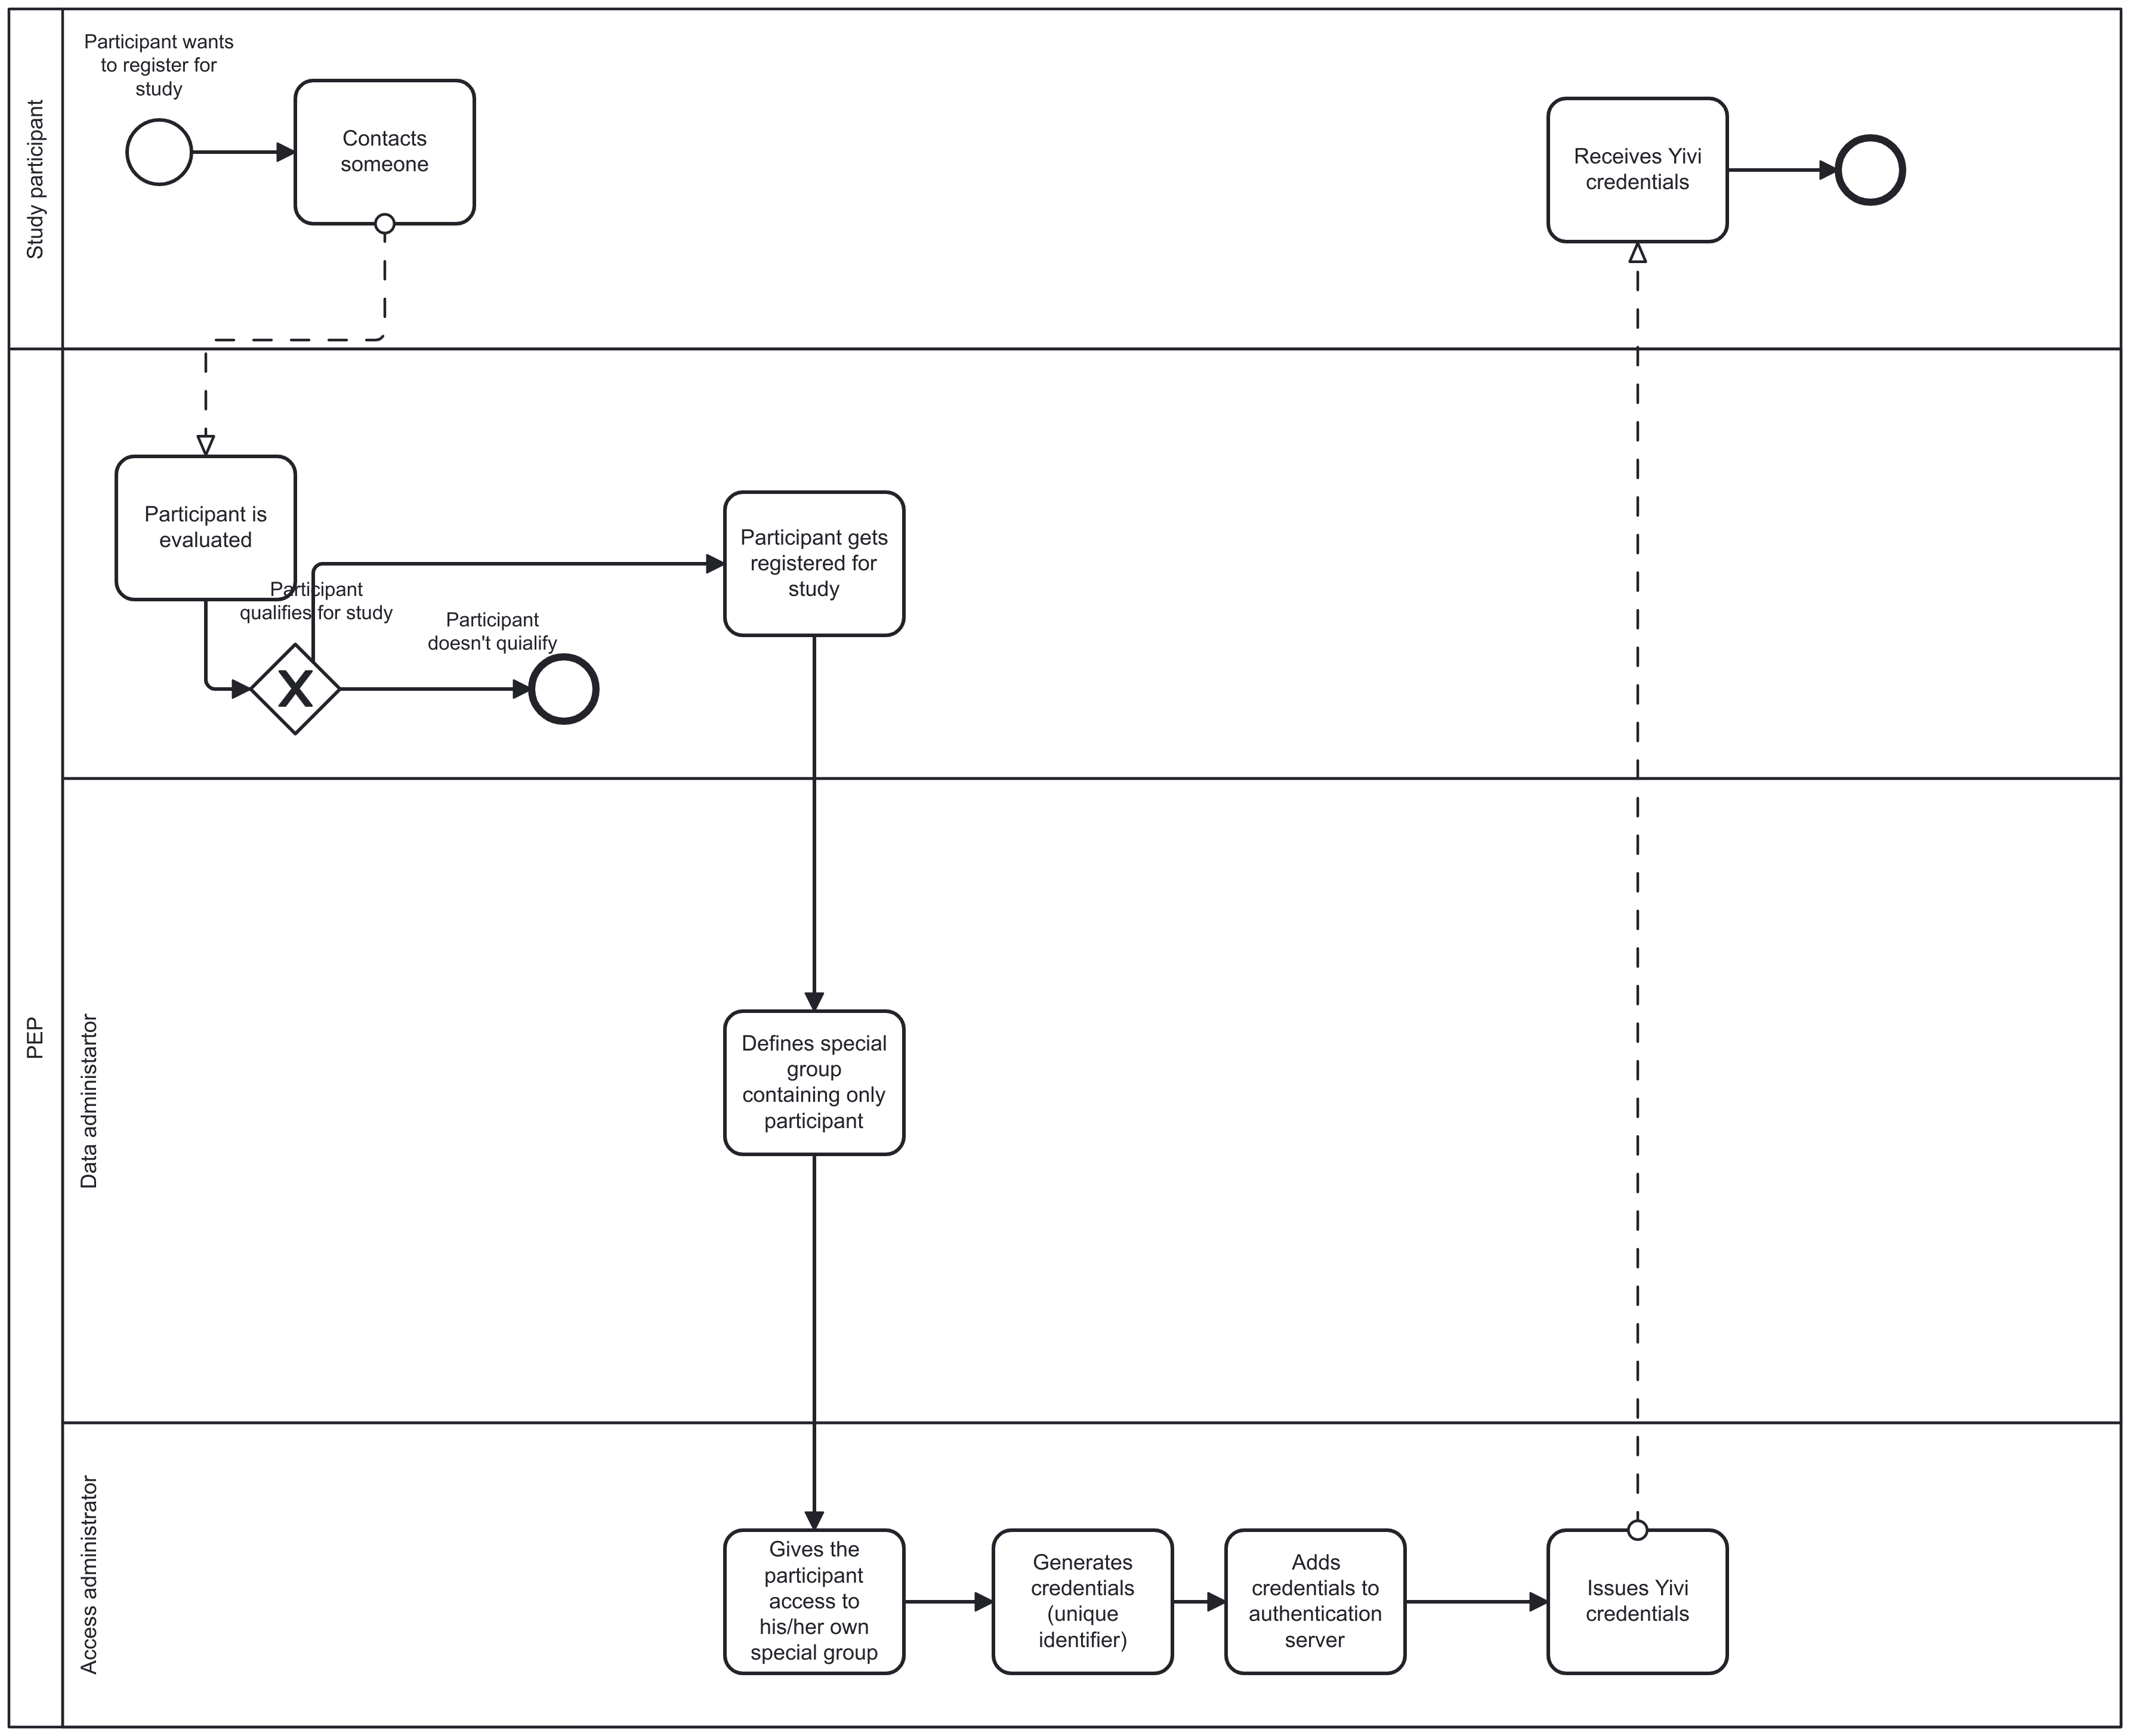
\includegraphics[scale=0.3]{registration_flow.png}
	\caption{Failed attempt registration flow as a BPMN diagram}
	\label{bpmn-registration-flow}
\end{figure}

Due to formatting constraints, the relative data access flow is available here \cite{data-access-failed-attempt-bpmn-diagram}.

This solution requires to generate a credential that lets a study participant authenticate to PEP, but without leaking the participant's identity. To be in line with PEP's own
design choices, I decided to use the string "participant:" followed by a random string as an identifier that gets linked to the participant during the registration phase. Such string is 
a version 4 UUID as described in RFC 4122 \cite{uuid_rfc}.  

\subsubsection{Version 4 UUID}
A version 4 UUID is a 128 bits-long value, usually represented as a string of hyphen-separated hexadecimal values. 6 bits are set to predetermined values, this leaves 122 bits of
randomness. "Do not assume that UUIDs are hard to guess; they should not be used
   as security capabilities (identifiers whose mere possession grants
   access), for example.  A predictable random number source will
   exacerbate the situation."

   do note that mere knowledge of the UUID doesn't grant access: one needs an YIVI card, so the attribute needs to be validated.

   \subsubsection{Estimating collision probability: the birthday paradox}\todo{Re-read everything and rewrite better e.g. by putting p=, pbar= etc}
To analyze the probability of two version 4 UUIDs colliding, we use the birthday paradox. 
What is the probability that two or more people share the same birthday in a group of $n$ people? 
To answer this question, it is easier to first compute the probability that no one has the same birthday, and then compute the complement probability. We start by ordering all the
people in the group, and then for each of them we ask what is the probability that that person doesn't share its birthday with any of the previous ones. For the first person, the
probability is 1, since we are not considering any other person yet. Then, the probability of the second person not sharing their birthdy with the previous one is the probability
that this person is born in any day of the year other than the day the first person was born in: $1-\frac{1}{365}$. For the third person, the probability of not sharing the
birthday with any of the previous two is the probability of being born in any day other than the two days already taken by the first two: $1-\frac{2}{365}$. This pattern stays
valid for any number $n$ of people\footnote{Some explanations of the problem define a special case for $n>365$. Although one can save computations by noting that if you have more
people than days in a year then you must have a collision, the general formula still works since one of the factors becomes zero.}, so the probability that in a group of $n$ people no-one shares its birthday with
another person of the same group is $1(1 - \frac{1}{365} ) \dotso  (1 - \frac{n - 1}{365} ) = \prod_{k=1}^{n-1}(1-\frac{k}{365})$. From this follows that the probability of having at least
to people that share their birthday in a group of $n$ people is

$$1-\prod_{k=1}^{n-1}(1-\frac{k}{365})$$

This result can be generalized to obtain a formula we can use for the case of version 4 UUID collisions. Instead of considering birthdays, let's consider the case of a group of $n$
people randomly choosing an object from a set of $u$ objects, with replacement. Here $u$ is the set of all possible version 4 UUIDs. Following the same reasoning as before, we obtain
$1(1-\frac{1}{u}) \dotso (1-\frac{n-1}{u}) = \prod_{k=1}^{n-1}(1-\frac{k}{u})$. So the probability of having at least two version 4 UUIDs colliding is

$$1- \prod_{k=1}^{n-1}(1-\frac{k}{u})$$

Computing the exact value for large values of $n$ and $u$ is prohibitive. For this reason, it is often used an approximation of the above formula. To derive it, we have to look at the
problem from a slightly different perspective. To see if there are collisions, we can look at all possible UUID pairs, and ask for each pair if the two UUIDs are the same or not.
Each comparison is a Bernoulli trial, so when we consider a sequence of such comparisons we obtain a binomial distribution. The probability of each pair not being a collision is
$\frac{1-u}{u}$. Since each Bernoulli trial is independent from the others, to get the probability of not having collisions in the set of all possible pairs, we can raise the
previous result to a power representing the cardinality of the set of all possible pairs: $(\frac{1-u}{u})^{\binom{n}{2}}$. From this, it follows that the probability of having at
least a collision is 

$$1-(\frac{1-u}{u})^{\binom{n}{2}}$$.

While rewriting the result in this form does not help computing it per se, we can now use the fact that this is a binomial distribution to apply a Poisson approximation. If we have
$n \geq 20$ and $p \leq 0.05$ or $n \geq 100$ and $p \leq 0.1$ a Poisson distribution of parameter $\lambda=np$ is a good approximation. Under this assumption, we can say that the
probability of not having collisions is $e^\lambda$ and the probability of having at least one collision is

$$1-e^\lambda$$

where $\lambda=np$.

Verion 4 UUIDs are 128 bits long, of which 122 are randomly generated. Assuming a uniformly random number generator is used, this gives us $u=2^122$ possible UUIDs. So we have $p=$


To implement this, I tried setting up SimpleSAMLphp \cite{simplesamlphp} to work as an YIVI \cite{about-irma} identity provider. SimpleSAMLphp can work both as a service provider and
as an identity provider, and can be extended by writing PHP plugins. There were already two previous attempts about writing such a plugin: 
"simplesamlphp-module-authirma" \cite{simplesamlphp-module-authirma} by the Privacy by Design Foundation \cite{privacybydesignfoundation} and "irma-idp" \cite{irma-idp} by SURF \cite{surf}.
Both appear to be unmaintained, but I first attempted to use those as a basis for my own implementation. \par
I started by setting up a local YIVI server inside a Docker container and creating a demo credential \cite{irma-docs-issuer} for PEP study participants, called "irma-demo.PEP.id". I
then tried making "simplesamlphp-module-authirma" work again. It was developed at a time where the YIVI HTTP server and the YIVI JSON API server where two separate components. While
trying to make it work again, I stumbled upon the problem of getting the keys for the API and web servers. Probably the key is the same for both, as now the irmago
server \cite{irma-docs-server} implements both, but I was not able to find the certificate in the required format inside my Docker container. \par
After failing to make "simplesamlphp-module-authirma" work again, I did some more research on previous work and found out about "irma-idp". It is more recent and, while it still
appears to be unmaintained, at least uses the current architecture where irmago provides both the HTTP server and JSON API server components \cite{irma-docs-server}. But this
project lacks configuration instructions and, again, I was not able to find the required certificate by trying the method reported in the repository's README \cite{irma-idp}. I asked 
for clarification in a GitHub issue, but to date I got no answer \cite{irma-idp-issue}. Additionally, looking at the code inside the repository it looked to either be incomplete or
contain an error: the HTML code inside the "disclose.html" file contains a "Verify attribute" button that does not do anything, and there is no way to trigger the redirect specified
inside the form. Likely the idea was to redirect the user upon clicking the aforementioned button, but in this case the code should have been written differently. \par
Since "simplesamlphp-module-authirma" is unmaintained and targeted an old YIVI server implementation, and "irma-idp" appears to be abandoned in a non-working state and with lacking
documentation, I decided to write my own SimpleSAMLphp plugin instead of adapting old projects to work with the new irmago implementation. This is because attempting to fix these
old implementations could have entailed a significant rewrite of their code, so I decided to start afresh. I installed and configured SimpleSAMLphp \cite{simplesamlphp-docs} as a SAML identity
provider \cite{sstc-saml-core-errata-2.0-wd-07} inside a Docker container, then I followed its documentation to write an authentication source talking with an YIVI server.
SimpleSAMLphp lets a developer write its own authentication flow. After authentication is completed, one has to pass to SimpleSAMLphp the relative attribute and it will take care
of generating a SAML assertion and send it to the user. Internally, it implements a state machine going through the different authentication steps. If a redirect is necessary
during the authentication flow, it is necessary to save the authentication state and then  restore it after the redirect. Since I had to show the user a custom page containing a QR
code to disclose its own YIVI credentials, I needed to save the state and perform a redirect. I could confirm the state was saved on a temporary file, but attempting to restore it
failed. It was likely a configuration error, but asking SimpleSAMLphp's developers for help didn't turn anything. After trying to fix this issue for some time I abandoned this
path. \todo{talk about registration component}

\iffalse

\subsection{Web application}
Everybody wants web apps! So let's give them what they want. After failing with SimpleSAMLphp, I 


\subsection{Some initial ideas}
The first idea to let users download their data from PEP was to use YIVI to disclose the data needed to generate the pseudonym to some component that then proceeds to generate it.
This doesn't work because the pseudonym is generated by encrypting a random string. But this string gets stored inside Salesforce, so the next idea was to interface with
Salesforce. This could have posed some issues though:
\begin{enumerate}
		\item Is the seed stored along some data that uniquely identifies the user?
		\item Does Salesforce have some API to interface with other software?
\end{enumerate}
Let's analyze these issues. If the seed is stored alongside personal data, then getting it from Salesforce could expose personal identifiable information. How? One could argue that
they shouldn't store anything inside Salesforce anyway... But it is done to be able to de-anonymize users in special circumstances. And here we get to the point: better not touch
Salesforce, unless those special circumstances arise. The second issue is about API access. Salesforce does have it, but only for certain editions \cite{salesforce}. The PEP team
blackballed the idea of accessing Salesforce. The next proposal was to give participants their own ID (main pseudonym) during the enrollment procedure as an YIVI credential, but
providing them with this ID could disclose more information than necessary.
Since this first idea was discarded, I considered the following approaches:
\begin{enumerate}
		\item Give participants their own ID during enrollment phase.
		\item Give participants a re-shuffled ID.
		\item Create a fake study in which the participant has the researcher role.
		\item Use YIVI’s chained session: it is possible to derive a card from other cards the user already has by having the user disclose he attributes contained there. The server can then apply some function on the attributes and derive a new card from that.
\end{enumerate}

The first approach could pose unnecessary risks. The participant's pseudonym is used to obtain the re-shuffled pseudnyms that identify the participant in different studies and in
different datasets. To be able to derive these pseudonyms, an attacker would also need to get the re-shuffle key, but not leaking the pseudonym outside of PEP in the first place would still be
better. \par
The second approach would solve the problem of leaking the participant's pseudonym, but participants would still need to be provided with some key material to ab able to decrypt
the data once downloaded. [Is this true though? Couldn't this just work the same as I have it implemented now?]. \par
In a similar fashion to the previous approach, it would be possible to create a fake study inside PEP with a single participant, one for each user. Then the users would be given
the researcher role inside their own fake study to be able to access their own data. Also this option would require to provide them with some key material, opening the door to keym
management issues [again, is this actually needed? See also previous note]. \par
The last approach is a way to sidestep the issue of providing study participants with their own pseudonym or a re-shuffled pseudonym. But it would require some way of linking the
YIVI identity to the participant.\par

\subsection{The chosen solution}
PEP uses rbac, let's use that too! First, create a column group containing all the columns pertaining to exam results. Then, for each participant, create a new participant group
containing only that participant. Create a new user and apply permissions as needed. And SBAM! You've got it! [Insert here actual participant enrollment procedure and provide
details].
\subsection{The pain of implementing the solution}
\fi


\printbibliography
\end{document}
